
\documentclass[12pt]{memoir}
\def\nsigla{MATH605C}
\def\nsiglahead{Elliptic Curves}
\def\nsemestre{SP}
\def\nyear{26}
\def\nterm{SP}
\def\nprofesor{Rachel Pries}
\def\nextra{Handout}
\def\nlang{ENG}

\input{../../../headerVarillyDiff}

% Fix numbering for memoir class without chapters
\renewcommand{\thesection}{\arabic{section}}
\renewcommand{\thefigure}{\arabic{figure}}

\begin{document}

\section{Objective and Introduction}

\begin{itemize}
    \item \textbf{Objective}\\ 
    Prove \(\int_{\ov{\cM}_{1,1}}\psi = 1/24\).
    
    Because we cannot compute this directly on the moduli space, we will instead pull the $\psi$ class back to a family of pointed elliptic curves. By integrating the pullback, we can determine the integral over the moduli space!

     \item \textbf{The Integral Map and Chow Groups}\\
The integral is the pushforward of the constant map:
\[
X\xrightarrow[]{c}\pt\quad\To\quad A^\ast(X)\xrightarrow[]{c_\ast=\int_X}A^\ast(\pt).
\]    
Only cycles with top codimension part have non-zero integrals. In essence, the integral captures the degree of that part.

\begin{center}
% https://tikzcd.yichuanshen.de/#N4Igdg9gJgpgziAXAbVABwnAlgFyxMJZABgBpiBdUkANwEMAbAVxiRAB124YdgAzANQ4A5ok4ACHJyxhOAIwAKAPQCMAXxBrS6TLnyEUZFVVqMWbThBowATgxkxgnAMYBVNQH1gK0us3aQDGw8AiIfY2p6ZlZEDnYrW3swRxcAWU9vXw0tHWD9MPITKPNY+WUVDxx-XL1QlAAmXyKzGLi0KpzA3RCDZAAWQsiWtgBBJU46OBwACjLVSoBKaq68uv6moejR8fZJmctrOwcndmd0r3C1Jc6g2t6AVg3TLdixianZ9nbrkxgoYXgRFAfBsEAAtkgfCAcBAkI0QAw6HIYAwFN18rEbFhhAALDoBEHgpBkaGwxAAZk2JTaWGWhIhFOoMLhVNanDBTEQknZdDQUwg4mQnDQWCUwAAtOppjgFhQQNREcjUei6iAsbj8cDQQySczEFDFSi0asDGrsXi6dqkJTScTqMiwFAkOKAGwAdlZbDQHhU8oRSKNKtN6otnXpLNt+vtMEdSHdntKXGElqJiHheoGz2pzj9huVJrYIc1IHDjMjmeKbPYeAYsGAzmyBKtiEekY9WarNdg4mcHneOHEAF5xNIwDgvHM-GHmy6mWT25W2L3+4PR+OTgkjskTmcMpcNAqA-m7oXzcXS7PI63F4mOTs9poKGogA
\begin{tikzcd}
\set{f+tg:\ t\in\bP^1} \arrow[r, "\pi"] \arrow[d] & \bP^1_t \arrow[d, "{\mu: t\mapsto [\pi^{-1}(t)]}"'] \arrow[l, "p_1"', bend right=67] \arrow[rd, "\tilde{c}"] &     &  & A^\ast(\bP^1_t) \arrow[rd, "\tilde c_\ast = \int_{\bP^1}"]                                              &             \\
{\overline{\cU}_{1,1}} \arrow[r]                  & {\overline{\cM}_{1,1}} \arrow[l, "\sg", bend left=67] \arrow[r, "c"']                                        & \pt &  & {A^\ast(\overline{\cM}_{1,1})} \arrow[r, "{c_\ast=\int_{\overline{\cM}_{1,1}}}"'] \arrow[u, "\mu^\ast"] & A^\ast(\pt)
\end{tikzcd}
\end{center}

From here, \(\int_{\ov{\cM}_{1,1}}\psi=c_\ast(\psi)=\tilde{c}_\ast(\mu^\ast(\psi))=\int_{\bP^1}\mu^\ast(\psi)\).
\item \textbf{The Psi Class}\\
The $\psi$ class in $\overline{\mathcal{M}}_{1,1}$ is the first Chern class of the relative cotangent line bundle associated to the mark $p_1$: $\psi = c_1(\mathbb{L}_1)$.

\item So we may outline how we're going to complete our objective:
\begin{enumerate}
    \item Create a family of elliptic curves.
    \item Describe the pullback of \(\psi\) in our family. 
    \item Describe the classifying map into \(\ov{\cM}_{1,1}\).
    \item Integrate it and verify the result.
\end{enumerate}
\end{itemize}
\vfill
\newpage
\section{Creating a Family}
Consider a family of cubics \(\cE\xrightarrow{\pi} \bP^1_{t}\) given by the pencil \(\set{f + tg = 0}\) with \(t \in \mathbb{P}^1\) where
\[
\left\lbrace
\begin{aligned}
&f = x^3 - 4x + 0.01y\\
&g = y^3 - 4y + 0.02x
\end{aligned}
\right.
\]

which pass through\footnote{For numerical reasons, they don't pass exactly through these points but very close.} the lattice points \((-2,2),(0,2),(2,2),\dots, (2,-2)\). By picking one of them, we get a family of elliptic curves with a mark determined by the chosen point.

\begin{figure}[h]
    \centering
    \begin{minipage}[t]{0.45\textwidth}
        \centering
        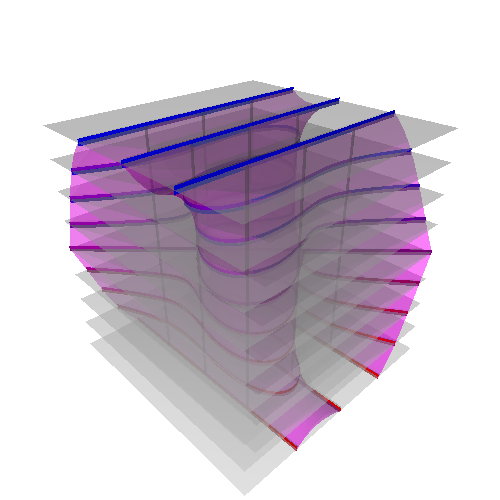
\includegraphics[width=\textwidth]{figs/cubic-family.png}
        \caption{$\{f+tg: t \in \bP^1\}$ with $t$ varying in the vertical direction}
    \end{minipage}%
    \hfill
    \begin{minipage}[t]{0.45\textwidth}
        \centering
        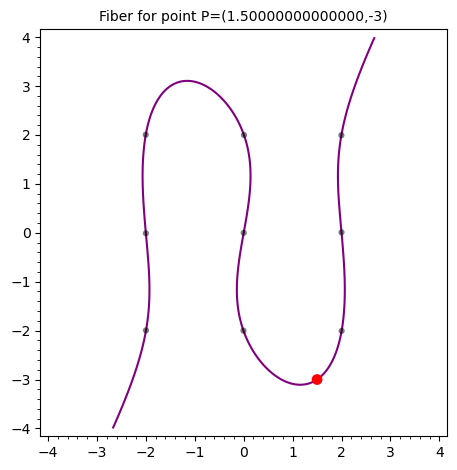
\includegraphics[width=\textwidth]{figs/particularFiber.png}
        \caption{Typical fiber at \(t = -0.177354709418838\)}
    \end{minipage}
\end{figure}



\begin{Ej}
    Via Bézout's theorem, verify that two cubics in general position intersect at exactly 9 distinct points.
\end{Ej}

\begin{Ej}
    Via the genus-degree formula \(g=\binom{d-1}{2}\), verify that all smooth curves in our family have genus one (and thus, are elliptic).
\end{Ej}

\begin{Ej}
    Convince yourself that choosing one of the intersection points \(p_i\) defines a section \(p_i:\bP^1_t\to \cE\), framing this as a family of pointed elliptic curves.
\end{Ej}

\begin{Ej}
    Draw the tangent to the fiber at \((0,2)\). Transport that drawing to the family. Convince yourself that the relative tangent bundle to the curves at the section is the same as the normal bundle of the section.
\end{Ej}
\section{Describing the Classifying Map}
Our family induces a classifying map 
\[
\mu: \mathbb{P}^1 \to \overline{\mathcal{M}}_{1,1},\quad t \mapsto [\pi^{-1}(t)],
\] 
which maps smooth/singular curves to smooth/singular points in the moduli space\footnote{Strictly speaking, this is the induced map at the level of families.}. The locus of singular curves forms an irreducible boundary divisor \(\dl_{\text{irr}}\subset\ov{\cM}_{1,1}\). Since all singular fibers map to this divisor, we can read the degree of $\mu$ simply by counting them. We count them as follows.

\begin{Ej}
The total space $\cE$ is the blowup of $\mathbb{P}^2$ at the 9 common points. Calculate its Euler characteristic $\chi(\mathcal{\cE})$ via \emph{additivity over disjoint unions}:
\[
\chi(\cE) = \chi(\bP^2)-9\cdot\chi(\pt)+9\cdot\chi(\bP^1)=\underline{\hspace{1cm}}-9\underline{\hspace{1cm}}+9\underline{\hspace{1cm}}=\underline{\hspace{1cm}}.
\]
\end{Ej}

\begin{Ej}
    Find the Euler characteristic of a nodal cubic:
    \[
    \chi(\text{nodal})=\chi(\bP^1)-2\chi(\pt)+\chi(\pt)=\underline{\hspace{1cm}}-2\underline{\hspace{1cm}}+\underline{\hspace{1cm}}=\underline{\hspace{1cm}}.
    \]
\end{Ej}

\begin{Ej}
    Via the \emph{multiplicativity over fibrations} for the Euler characteristic, \(\chi(\cE)=\chi(F)\chi(B)\), realize that:
    \[
    \chi(\cE)=(\text{number of singular fibers})\cdot\chi(\text{nodal}).
    \]
    From this, find the degree of the map \(\mu\) via the previous exercise.
\end{Ej}

\section{Final Computation}
To compute the final integral, we use everything we've gathered up to now. Explicitly, we need:
\[
\psi_1=-c_1\left(\cO_E(E)\right)=-(-\pt).
\]
and the fact that the map from the coarse moduli space \(\overline{M}_{1,1}\) to the stack \(\ov{\cM}_{1,1}\) has degree 2.

\begin{Ej}
    Fill in the blanks to complete the proof:
\[ 
\int_{\overline{\mathcal{M}}_{1,1}} \psi = \frac{1}{2\deg(\mu)} \int_{\mathbb{P}^1} \mu^* \psi =\frac{1}{2\cdot(\underline{\hspace{1cm}})}\int_{\bP^1}\underline{\hspace{1.5cm}}=\underline{\hspace{1.5cm}}.
\]
\end{Ej}


\end{document}
